\documentclass{article}
\usepackage[T1]{fontenc}
\usepackage{lmodern}
\usepackage{graphicx}
\usepackage{amsmath,amssymb}
\usepackage[a4paper,margin=2cm]{geometry}
\usepackage[absolute,overlay]{textpos}
\setlength{\TPHorizModule}{1mm}
\setlength{\TPVertModule}{1mm}
\usepackage[indonesian]{babel}
\usepackage{hyperref}
\setlength{\emergencystretch}{2em}
% unit: Halaman 4

\begin{document}

% === Halaman 4 (llm) ===

Fakta: Gambar-gambar bertebaran di internet
(website, social media, social networking)

\vspace{10mm}

% deskripsi: Screenshot postingan Facebook oleh Yogi Wahyu Prasida tentang kecelakaan kecil taksi otonom di Singapura.
% bbox normalisasi: [0.1520, 0.2780, 0.4780, 0.9250]
\begin{textblock*}{68.46mm}(31.92mm,82.57mm)
\noindent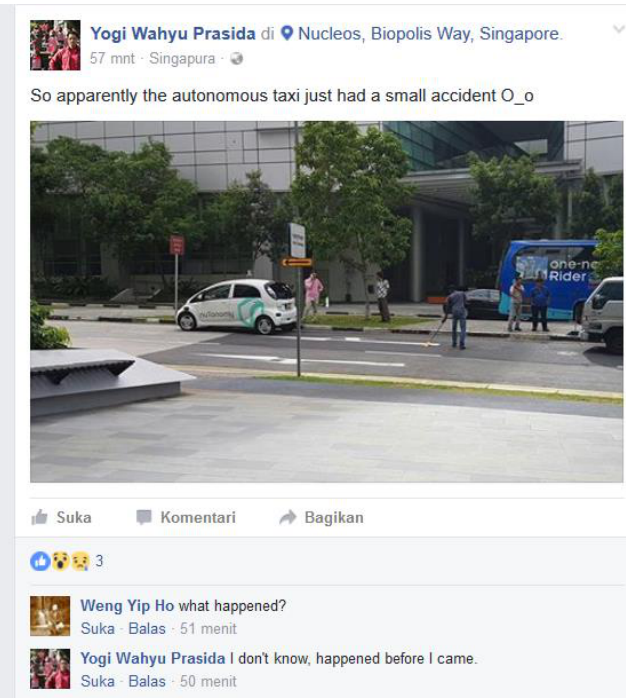
\includegraphics[width=68.46mm,height=192.16mm]{../../images/llm/page_004_img_01.png}%
\end{textblock*}

% deskripsi: Screenshot postingan Instagram oleh ashleyyukki yang menampilkan foto Jembatan Golden Gate.
% bbox normalisasi: [0.5780, 0.2780, 0.7840, 0.9320]
\begin{textblock*}{43.26mm}(121.38mm,82.57mm)
\noindent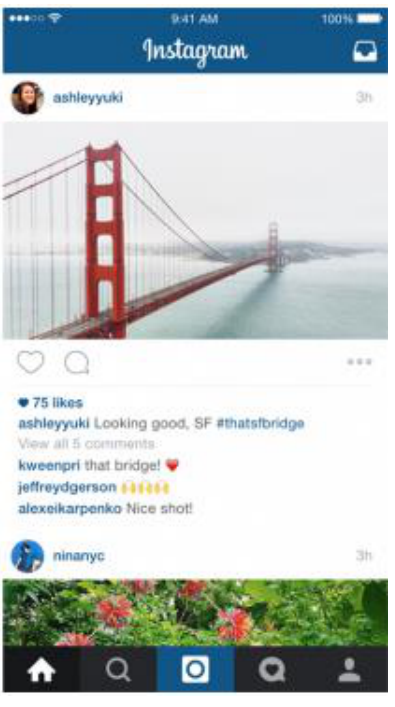
\includegraphics[width=43.26mm,height=194.24mm]{../../images/llm/page_004_img_02.png}%
\end{textblock*}

\end{document}
